\documentclass[a4paper, 11pt]{article}
%\usepackage[top=3cm, bottom=3cm, left = 2cm, right = 2cm]{geometry} 
%\geometry{a4paper}
\usepackage[utf8]{inputenc}
\usepackage{textcomp}
\usepackage{float}
\usepackage{graphicx}
\usepackage{parskip}
\usepackage{subfiles}
\usepackage{amsmath,amssymb}  
\usepackage{todonotes}
\usepackage[english]{babel}
\setlength {\marginparwidth }{2cm}
\usepackage{bm}  
\usepackage[pdftex,bookmarks,colorlinks,breaklinks]{hyperref}  
\hypersetup{linkcolor=black,citecolor=black,filecolor=black,urlcolor=black}
\usepackage{memhfixc} 
\usepackage{pdfsync}  
\usepackage{fancyhdr}
\pagestyle{fancy}
\setlength{\headheight}{14pt}
\bibliographystyle{plain}
\usepackage{listings}
\definecolor{backcolour}{RGB}{240,240,240}

\lstdefinestyle{mystyle}{
    backgroundcolor=\color{backcolour},   
    basicstyle=\ttfamily\tiny,
    breakatwhitespace=false,         
    breaklines=true,                 
    captionpos=b,                    
    keepspaces=true,                 
    showspaces=false,                
    showstringspaces=false,
    showtabs=false,                  
    tabsize=2
}
\lstset{style=mystyle}
\begin{document}

\begin{titlepage}
	\begin{center}
		
\includegraphics[scale=0.1]{images/unipd_logo.png}\\		
		\vspace{4\baselineskip}
		\Huge Wireless Networks for Mobile Applications\\
        \vspace{4\baselineskip}
		\LARGE Exam Project: \\
        Real-time crowd information using Bluetooth in a cloud-oriented architecture\\
		\vfill
		Author: Marchiori Luca - 2090458\\
	\end{center}
\end{titlepage}


\tableofcontents

\newpage
\section{Introduction}
Understanding occupancy levels in buildings and rooms has become increasingly valuable in various contexts. One significant application is assessing the availability of seating in libraries that do not have booking systems in place. By knowing the number of people currently present in the library, individuals have a way of knowing the probability of finding an open space to study or work. 

Monitoring occupancy levels is crucial for effective workforce management: for businesses with multiple stores or offices, having real-time data on the number of people in each location allows management to allocate the appropriate amount of personnel accordingly. This ensures that staffing levels match customer demand or operational requirements, improving productivity and customer service.

In the event of a pandemic or other health-related concerns, understanding occupancy levels is critical for enforcing safety measures and organizing access to various places. By monitoring the number of individuals in a building or room, establishments can maintain social distancing protocols, manage crowd control, and implement measures to prevent overcrowding or potential outbreaks. Finally, in case of an emergency, it can be useful to get to know the amount of people in buildings to organize the rescue accordingly.

Tracking occupancy in buildings, especially those without strict entrance controls or booking systems, can indeed pose challenges. However, there are potential solutions to estimate occupancy even without exact tracking capabilities.

One approach could be leveraging the diffusion of Bluetooth technology in today's society. With most individuals carrying at least one device with Bluetooth capabilities, such as smartphones or other connected devices, a continuous Bluetooth scan can be conducted to estimate the number of devices present in a room. While this method may not provide an exact count of people, it can still offer a useful estimation and indicate the overall occupancy trends throughout the day. By calculating the average number of active Bluetooth devices carried by an individual, it becomes possible to estimate the number of people in an area. 

This project aims to develop a system that utilizes Bluetooth technology to display the approximate number of devices in a room over a certain period of time. The system would conduct continuous Bluetooth scans, tally the number of active devices, and present this data to provide insights into the occupancy patterns. By implementing such a system, organizations and individuals can have a better understanding of real-time occupancy levels, enabling them to make informed decisions about resource allocation, crowd management, and safety measures.

\newpage
\section{System architecture}
The system architecture of the project is divided into two main units: the scanner devices and the server. The server itself is divided into a backend and a frontend applications.

The scanner devices are deployed as independent units. Each scanner consists of a single-board computer that performs periodic scans of the Bluetooth network, detecting all available devices within its range. Once the scanning routine is completed, the device sends the collected data to the backend of the centralized server via an HTTP POST request to a specific API endpoint.

The backend of the server functions as a web server. It receives the requests from the scanner devices, processes the data, and stores it into a database. Additionally, the backend handles GET requests from the frontend application: it retrieves the requested data by querying the database and provides it as a response to the frontend.

On the other hand, the server frontend serves as an interface between the user and the entire system. It provides webpages that can be accessed by users to interact with the system. The frontend can also trigger API requests to the backend server, requesting specific data. This data is then organized and presented to the user in a graphical view, enhancing the user experience.

Overall, this system architecture ensures that the scanner devices can operate autonomously, collecting data and sending it to the central server. The server backend handles data processing, storage, and retrieval, while the frontend enables user interaction and presentation of the collected data in a user-friendly manner. The following scheme summarize the architecture and the data flow.

\begin{figure}
    \centering
    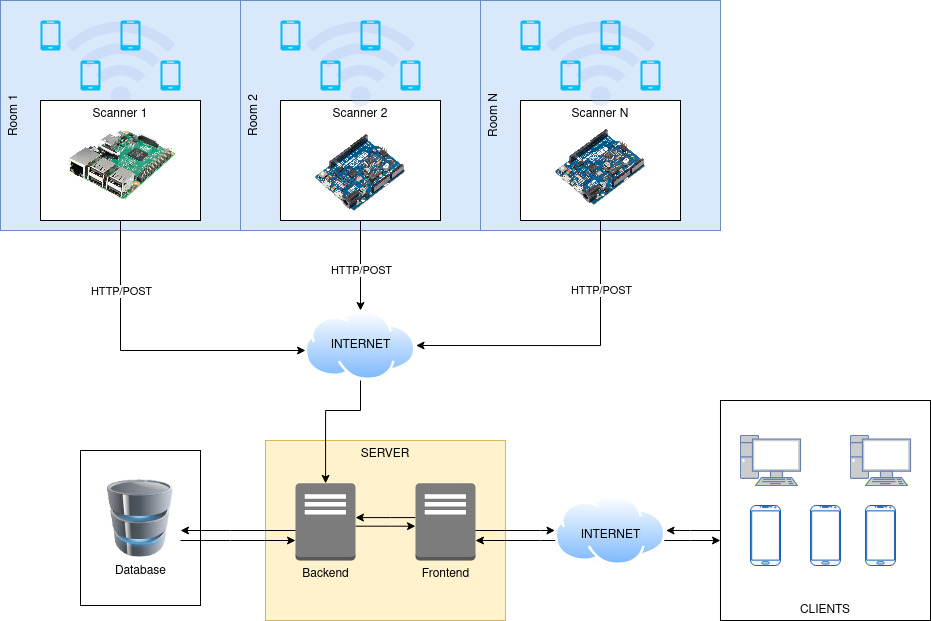
\includegraphics[width=1\linewidth]{images/WNMA-ProjectScheme.jpg}
    \caption{Project architecture}
    \label{fig:enter-label}
\end{figure}



\newpage
\section{Technologies}
\subsection{Hardware devices}
To implement the proposed system for tracking occupancy using Bluetooth scans, single-board computers like Raspberry Pi \cite{RPI} and Arduino \cite{arduino} are suitable choices. 

The devices used in this system need to have Bluetooth capabilities, allowing them to scan for nearby devices and gather occupancy data. Additionally, they should be capable of connecting to the internet either through WiFi or Ethernet to transmit the collected data to a server for storage and analysis. To facilitate the deployment process, these devices should be compact in size, making it easier to install them in various rooms and buildings and, considering the infrastructure cost, it is desirable to opt for inexpensive devices.

Both the Raspberry Pi and the Arduino, known for its versatility and functionality, fits the criteria effectively. They provides Bluetooth capabilities and options for internet connectivity through WiFi or Ethernet and their compact form factor allows for convenient deployment.

For this project due to board availability, a Raspberry Pi 3B+ has been used. However, since the logic is written in the Go programming language \cite{golang}, the exact same source code can be compiled with Tiny Go \cite{tinygo} \footnote{TinyGo is a Go compiler intended for use in small places such as microcontrollers, WebAssembly (wasm/wasi), and command-line tools.} to be run on Arduino or similar devices.

\subsection{Bluetooth}
Bluetooth is a wireless communication technology that allows devices to exchange data and connect with each other over short distances. It uses radio waves in the 2.4 GHz frequency range to establish a secure and low-power connection between devices.

Even though Bluetooth enables the sharing of data, in this project it is only used the scanning capabilities of this technology. When the scanner starts the discovery routine it sends out inquiry messages to discover other Bluetooth devices in its vicinity. These messages are broadcasted using 2.4 GHz. Bluetooth devices that receive the inquiry message can respond with their information, including their unique identifier called the Bluetooth device address or MAC address. The scanning device can also measure the Received Signal Strength Indication (RSSI) of the responses. RSSI provides an estimate of the signal strength between the scanning device and the responding devices. This information can be used to estimate the proximity or distance between devices, or in this project can be used to exclude devices outside the room (or building). 

Bluetooth Low Energy (BLE) is a subset of Bluetooth designed for low-power applications. The main differences between Bluetooth and BLE are power consumption, data transfer rates, range, and application focus. Bluetooth consumes more power, offers higher data transfer rates, has a longer range, and is suitable for continuous data streaming. BLE is optimized for low power consumption, has lower data transfer rates, has a shorter range, and is suitable for intermittent communication in devices with limited power resources. Both Bluetooth and BLE can coexist and support interoperability between devices.

This projects, using the go-bluetooth library, enables the scanning of both Bluetooth and Bluetooth Low Energy devices, allowing for scanning not only smartphones and computer but also smalls devices such as earphones, smart pencils, peripherals and watches.

\subsection{Programming languages and frameworks}
\subsubsection{Go}
Go, also known as Golang, is a compiled, statically typed, and open source programming language that has gained popularity for building microservices and cloud architectures. It is developed and mainteined by Google. In this project, both the server and the scanner logic are written in Go.

\textbf{Scanner}\\
One of the reasons for choosing Go for the scanner devices is its excellent run-time efficiency. It allows the scanner code to run smoothly even on low-power hardware like single board computers. Furthermore, Go can be compiled with the gc compiler to run on Linux with ARM processors, making it a suitable choice for devices like Raspberry Pi. Additionally, Go can be compiled with the tinygo compiler to run on embedded systems and microcontrollers such as Arduino.

To facilitate the interaction with Bluetooth devices on Linux systems, the go-bluetooth library \cite{go-bluetooth} has been used in this project. This library acts as a wrapper to the Bluez DBus API and offers high-level APIs that simplify the process of communicating with Bluetooth devices on Linux-based systems.

\textbf{Server}\\
For the server component of this project, Go was chosen due to its capability to support the development of web applications. The language provides a range of useful tools, including an integrated web server provided by the http package \cite{go-http} in its standard library. This allows to quickly set up and deploy web APIs that are used to receive data from scanners and provide data to the front end.

\subsubsection{React / JS}
React \cite{react} is a highly popular and widely used front-end JavaScript library that enables developers to build user interfaces based on reusable components. It is an open-source project maintained by Meta.

One of the key advantages of using React is its ability to create single-page applications, mobile applications, or server-rendered applications in conjunction with frameworks like Next.js. This flexibility allows developers to build applications for various platforms and use cases.

In this project, the frontend has been developed using React. By leveraging React's component-based architecture, it was possible to create reusable UI components that can be easily composed to build more complex user interfaces. This results in cleaner and more maintainable code and the possibility to easily expand the project with more features.

To implement the data visualization pages, the Chart.js library \cite{chartjs} has been used. This library provides powerful charting and graphing functionalities, allowing the presentation of data in a visually appealing and informative manner.

For handling API calls to the backend, the project utilizes the Axios library \cite{axios}. Axios simplifies the process of making HTTP requests and handling responses, providing a convenient and efficient way to interact with the backend server.

\subsection{Database}
The server implements SQLite \cite{sqlite} as its database system. SQLite belongs to the family of embedded databases, which are database management systems tightly integrated with an application software, avoiding the need for external servers. SQLite is widely deployed and used by top web browsers, operating systems, mobile phones, and other embedded systems.

The decision to use SQLite in this project was based on its embedded nature, as it enables faster development and deployment. SQLite stores the database in files that can be easily managed and deployed, eliminating the need for complex server setups and heavier (DBMS). This simplicity and portability make SQLite an ideal choice for this prototype.

However, it's worth noting that SQLite can be easily replaced with more powerful DBMS options such as MySQL or PostgreSQL, depending on the specific requirements and scalability needs of the project. These DBMSs offer additional features and can handle larger, more complex databases if necessary. For the purposes of this project, SQLite provides an efficient and practical solution.

\newpage

\section{Development}
\subsection{Scanner}
The scanner's main function consists on simply two task: run the Bluetooth device scan and posting the data to the back-end web server.

\begin{lstlisting}[language=Go]
func main() {
	log.Infof("Bluetooth affluence script started")
	aid := adapter.GetDefaultAdapterID()
	scan, err := Run(aid, 60) // The scan is 60 seconds long
	
	if err != nil {
		log.Error(err)
		os.Exit(1)
	}

	err = postScanResults(scan)
	if err != nil {
		log.Error("Error sending data to server")
		os.Exit(1)
	}

	os.Exit(0)
}

\end{lstlisting}

The length of the scanning process is hard-coded to 60 seconds. Using a scan duration too little can lead to not having enough time to scan all the devices around, setting it to a high value can lead to record devices that already left the room.

The scanning routine, given the Bluetooth adapter id, execute first a power cycle of the adapter to be use that it is up and running, after that, it flushes its cache to avoid missing devices, finally it runs the scan, until a timer-thread signals the expiration of the scan timeout. In the end, it fills a Scan datatype and sends it to the server.

The Scan datatype contains the list of the scanned devices, along with thier names, aliases, RSSIs, etc. along with the information of the scan such as the scanner properties and the timestamp of the scan.

In the following code block it's reported a simplified version of the code of the scanning function. Here, error handling and other functionalities are missing for space-related needs. The full code is available in the linked Github repository \cite{repo}. 


\begin{lstlisting}[language=Go]
func Run(adapterID string, timer int) (Scan, error) {
	var devices []Device
	a, err := adapter.GetAdapter(adapterID)
	var s Scanner = ScannerProps(*a)
	PowerCycle(*a)
	err = a.FlushDevices()
	discovery, cancel, err := api.Discover(a, nil)

	go func() {
		time.Sleep(time.Duration(timer) * time.Second)
		cancel()
	}()

	for ev := range discovery {
		dev, err := device.NewDevice1(ev.Path)
		device := Device{Address: dev.Properties.Address, Alias: dev.Properties.Alias, Name: dev.Properties.Name, RSSI: dev.Properties.RSSI, TxPower: dev.Properties.TxPower}
		device.Alias, device.Name)
		addDevice(&devices, device)
	}

	dt := time.Now().Format(time.RFC3339)
	scan := Scan{Devices: devices, Scanner: s, ScanTime: dt}
	return scan, nil
}

\end{lstlisting}

After the scanning function, the content of the Scan is converted into Json and sent to the back-end server with a POST request.

This script can be set to run automatically by configure an utility such as Crontab to execute the script. Crontab is a command in Unix-like operating systems that allows you to schedule recurring tasks or commands to run automatically at specific time intervals. The Crontab syntax consists of six fields, specifying the minute, hour, day of the month, month, day of the week, and the command to be executed. These fields can be set to specific values or can use special characters and wildcards to match multiple values. For example, the following Crontab entry executes the command "runScan" every 5 minutes:
\begin{lstlisting}[language=Bash]
*/5 * * * * /path/to/runScan
\end{lstlisting}

By increasing the frequency of the scan, it is possible to increase the granularity of the data store. Note that it can never be less than the scanning timeout set in the script.

\subsection{Server back-end}


\subsection{Server front-end}
\newpage

\section{Tests}
\newpage

\section{Results}

\newpage
\begin{thebibliography}{9}
\bibitem{repo}
Project's GitHub repository - \href{https://github.com/lucamarchiori/BluetoothAffluence}{github.com/lucamarchiori/BluetoothAffluence}
\bibitem{golang}
\href{https://go.dev/}{The Go Programming Language}

\bibitem{tinygo}
\href{https://tinygo.org/}{Tiny-Go - Go on embedded systems}

\bibitem{RPI}
\href{https://www.raspberrypi.com/documentation/computers/raspberry-pi.html}{Raspberry Pi}

\bibitem{arduino}
\href{https://docs.arduino.cc/}{Arduino}

\bibitem{go-bluetooth}
\href{https://pkg.go.dev/github.com/muka/go-bluetooth@v0.0.0-20221213043340-85dc80edc4e1#section-readme}{go-bluetooth Library}

\bibitem{go-http}
\href{https://pkg.go.dev/net/http}{Go HTTP package (std lib)}

\bibitem{react}
\href{https://react.dev/}{React framework}

\bibitem{chartjs}
\href{https://www.chartjs.org/}{React JS charting library}

\bibitem{axios}
\href{https://axios-http.com/}{Axios - Promise based HTTP client}

\bibitem{sqlite}
\href{https://www.sqlite.org/index.html}{SQLite Database}
\end{thebibliography}
\end{document}